\documentclass[twocolumn,a4paper]{jsarticle}
%
\usepackage[dvipdfmx]{graphicx}
\usepackage{amsmath,amssymb}
\usepackage{bm}
\usepackage{ascmac}
\usepackage{listings} %日本語のコメントアウトをする場合jlistingが必要
%ここからソースコードの表示に関する設定
\lstset{
  basicstyle={\ttfamily},
  identifierstyle={\small},
  commentstyle={\smallitshape},
  keywordstyle={\small\bfseries},
  ndkeywordstyle={\small},
  stringstyle={\small\ttfamily},
  frame={tb},
  breaklines=true,
  columns=[l]{fullflexible},
  numbers=left,
  xrightmargin=0zw,
  xleftmargin=3zw,
  numberstyle={\scriptsize},
  stepnumber=1,
  numbersep=1zw,
  lineskip=-0.5ex
}
%
\setlength{\textwidth}{\fullwidth}
\setlength{\textheight}{40\baselineskip}
\addtolength{\textheight}{\topskip}
\setlength{\voffset}{-0.2in}
\setlength{\topmargin}{0pt}
\setlength{\headheight}{0pt}
\setlength{\headsep}{0pt}
%
\newcommand{\divergence}{\mathrm{div}\,}  %ダイバージェンス
\newcommand{\grad}{\mathrm{grad}\,}  %グラディエント
\newcommand{\rot}{\mathrm{rot}\,}  %ローテーション
%
\title{信号の無い交差点における車両の挙動のモデル化と検証}
\author{1955008	佐原優衣}
\date{}

\begin{document}
\maketitle

\section{システムモデル}
信号のない交差点における,自動運転車が通過可能かどうかを判断する中央制御システムをモデル化し,検証を行う。本稿では,自動運転車のみで,交差点を通過する際どのように通過可能かを判断する中央制御システムがあるとする。
本システムは,中央でどこからどこへ向かう車両が交差点を通過するか把握しており,その情報から,各車両が交差点進入可能かを判断する仕組みである。
今回の通過可能の判断は二段階式にした。まず,左右方向に車両がきていないことを確認し,次に前方車にぶつからないことを確認する形にした。
\section{UPPAALモデルの解説}
本モデルでは直進する車両のみをモデル化した。
\subsection{大域宣言}

clock		gc;

int dir03,dir30,dir12,dir21;

int count;

int way[4];

int cross[4];

大域時間変数gcと車両がどこからどこへ進むかを示す方向変数を用意し,交差点にいる全ての車両の台数を示すcount,一段階目の確認の時に参照する配列wayと二段階目の確認時参照するcrossを大域宣言とする。

\subsection{テンプレート}
本UPPAALモデルではテンプレートは車両のみである。
\subsubsection{車両テンプレートの局所宣言}
本テンプレートでは局所時間変数local\_clockと左右を確認するために自分の出発地から左右をはどこかを出す関数を作り局所宣言で記述する(図\ref{locdec})。
\begin{figure}
  \centering
  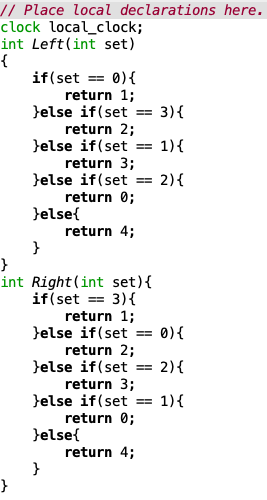
\includegraphics[width=40mm]{local_dec.png}
  \caption{車両のテンプレートの局所宣言}
  \label{locdec}
\end{figure}
\subsubsection{テンプレートの図}
\begin{figure}
  \centering
  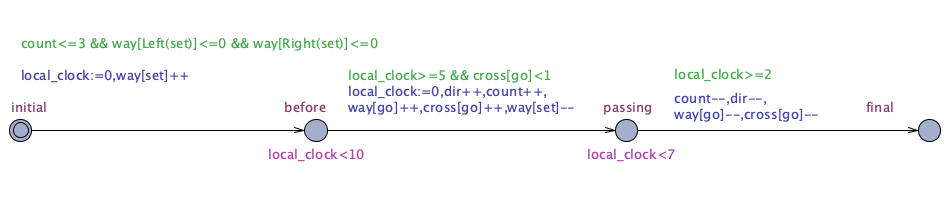
\includegraphics[width=75mm]{temp.png}
  \caption{車両のテンプレート}
  \label{temp}
\end{figure}
パラメータはどの方向の車両かを示すdecを宣言し,大域変数を参照し,各車両の始点終点を保持するset, goを宣言した(図\ref{temp})。
\subsection{システム宣言}
sn = AV(dir30, 3, 0);

sn2 = AV(dir30, 3, 0);

ns = AV(dir03, 0, 3);

ew = AV(dir12, 1, 2);

ew2 = AV(dir12, 1, 2);

we = AV(dir21, 2, 1);

system	sn,sn2,ns,ew,ew2,we;

南から北へ直視する車両をsnとsn2,その逆をns,東から西へ直進する車両をewとew2,その逆をwe,として宣言した。
\section{シミュレーション}
東から西へ直進するewが交差点を通過中で,西から東へ直進するweと東から西へ直進するew2が交差点に進入する時の状態がシミュレーション画面に表示されている(図\ref{simu})。その時可能な遷移はweとewだけである。cross配列3が1なのでew2が遷移できない(図\ref{able})。ewが遷移するまでew2はpassingローカルに遷移できないからである。

\begin{figure}
  \centering
  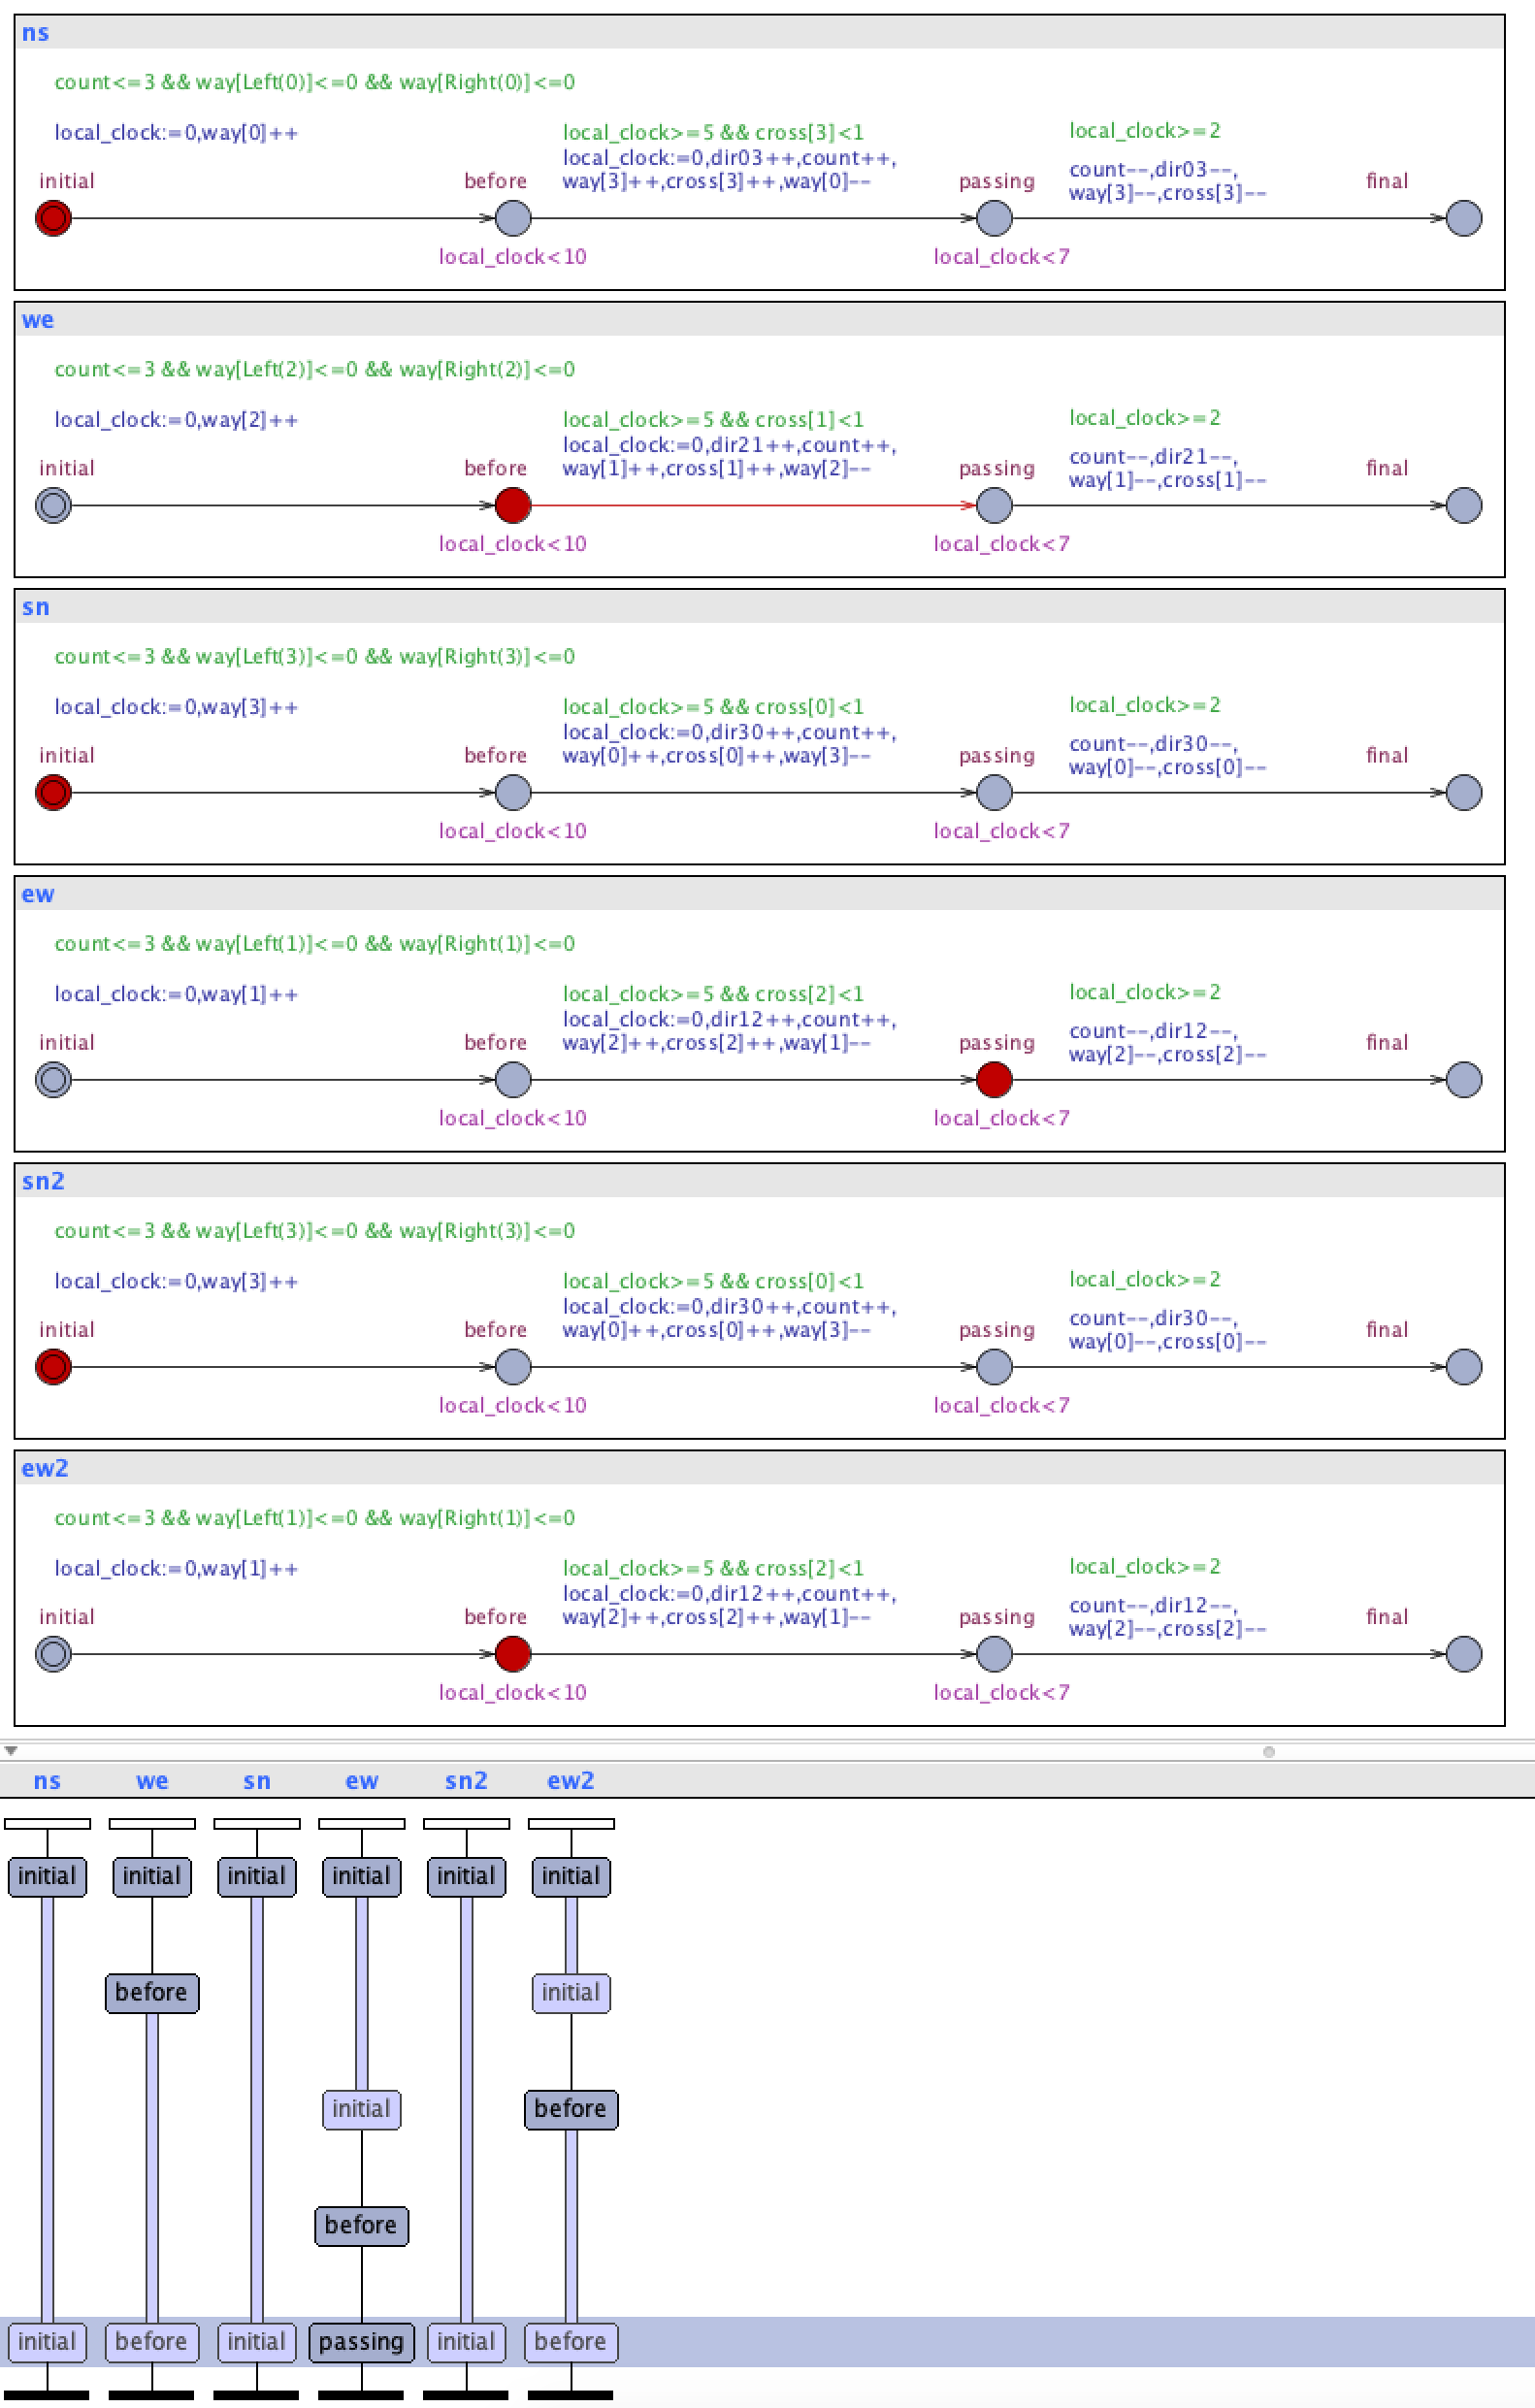
\includegraphics[width=60mm]{simu.png}
  \caption{シミュレーション画面}
  \label{simu}
\end{figure}
\begin{figure}
  \centering
  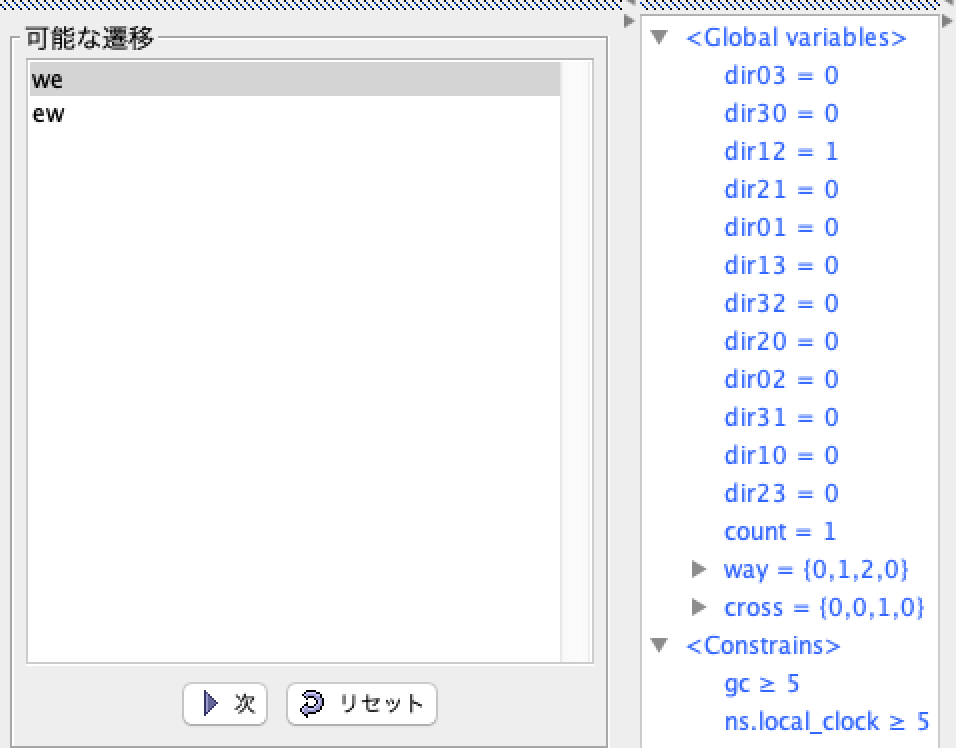
\includegraphics[width=50mm]{able.png}
  \caption{遷移可能な車両}
  \label{able}
\end{figure}

\section{検証}
6台の車両が交差点を通過終了する最小時間の検証を行う。
最小時間の検証は基本特性の到達可能性と安全特性を組み合わせて行う。
まず,到達可能性を検証し,その性質が満たされるならば,安全特性の検証を行う。そして,安全特性が満たされれば最小時間が算出できたことになり,満たされなければ最小時間ではないことがわかるため,再度,到達可能性の検証を行う。この一連を繰り返した結果,本モデルにおける最小時間は,18単位時間であることがわかった。
満たされた検証式を次に示す。

$E<>$ (gc==18 and (ns.final and we.final and sn.final and ew.final and sn2.final and ew2.final))



$A[]$ ($gc<18$ imply not (ns.final and we.final and sn.final and ew.final and sn2.final and ew2.final))

\section{まとめ}
直進する車両だけならば,進行方向が垂直な時は遷移不可で,かつ同方向で前方車がいるときの遷移不可になることを確認できた。また6台の通過最小時間は18単位時間だったので,前方車追従を行いながら,進行方向が平行な車両が同時に通過することによってこの値になったと考えられる。
\end{document}
\begin{itemize}
  \item item1
  \item item2
  \item ...
  \item itemN
\end{itemize}
文献\cite{key1}

\begin{thebibliography}{3}
  \bibitem{key1} 参考文献の名前・著者1
  \bibitem{key2} 参考文献の名前・著者2
  \bibitem{keyN} 参考文献の名前・著者N
\end{thebibliography}